\chapter{Rozwiązania implementacyjne}
  
  W poprzednim rozdziale opisano narzędzia jakie wykorzystano w trakcie budowy prototypu. W niniejszym rozdziale, przedstawiono zastosowane konkretne rozwiązania implementacyjne. Szczególną uwagę zwrócono na moduł edycji diagramów przypadków użycia oraz generator specyfikacji wymagań.

  \section{Architektura systemu}

    System Reqmanager zbudowany jest w oparciu o, opisaną w rozdziale 4, technologię Grails, integrującą wiele istniejących rozwiązań zbudowanych na bazie wirtualnej maszyny Javy. Na Rysunku \ref{fig:techstack} przedstawiono ogólną architekturę Grails.

    \begin{figure*}[h]
      \centering
      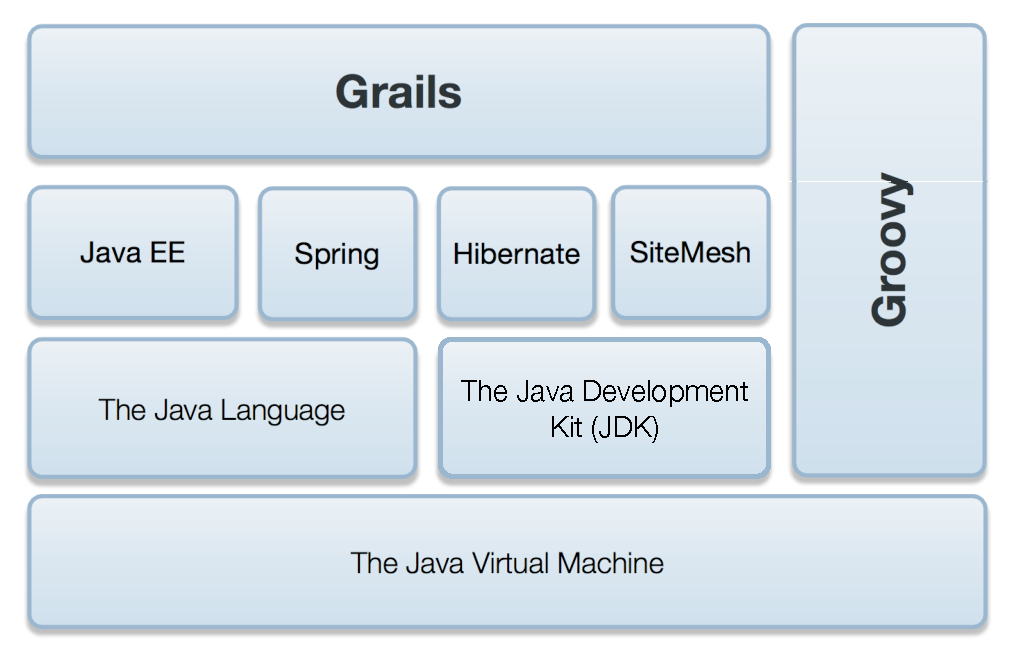
\includegraphics[width=1.0\textwidth]{img/grails-stack-rev2.pdf}
      \caption{Architektura Grails}
      \label{fig:techstack}
    \end{figure*}
     
    Definiowanie wymagań w systemie Reqmanager polega na jednoczesnym dostępie do edytora tekstu oraz edytora diagramów przypadków użycia. Użytkownik, mając otwartą aplikację, oprócz tekstowego opisu wymagania, ma możliwość dodawania oraz edycji przypadków użycia w formie graficznej.

    Aplikacja Reqmanager jest typową aplikacją internetową typu klient-serwer, gdzie klientem jest przeglądarka użytkownika korzystającego z aplikacji zainstalowanej na zdalnym serwerze, odpowiednio reagującej na żądania klienta na zasadzie żądanie - odpowiedź (request - response). Przeglądarka internetowa jest tak zwanym ,,cienkim klientem'' z racji silnego uzależnienia działania od serwera aplikacji. Na Rysunku \ref{fig:reqarch} przedstawiono poszczególne moduły proponowanego systemu wraz z podziałem na warstwy.
 
    Na potrzeby aplikacji Reqmanager, utworzono następującą strukturę modeli aplikacji:

    \begin{figure*}[p]
      \centering
      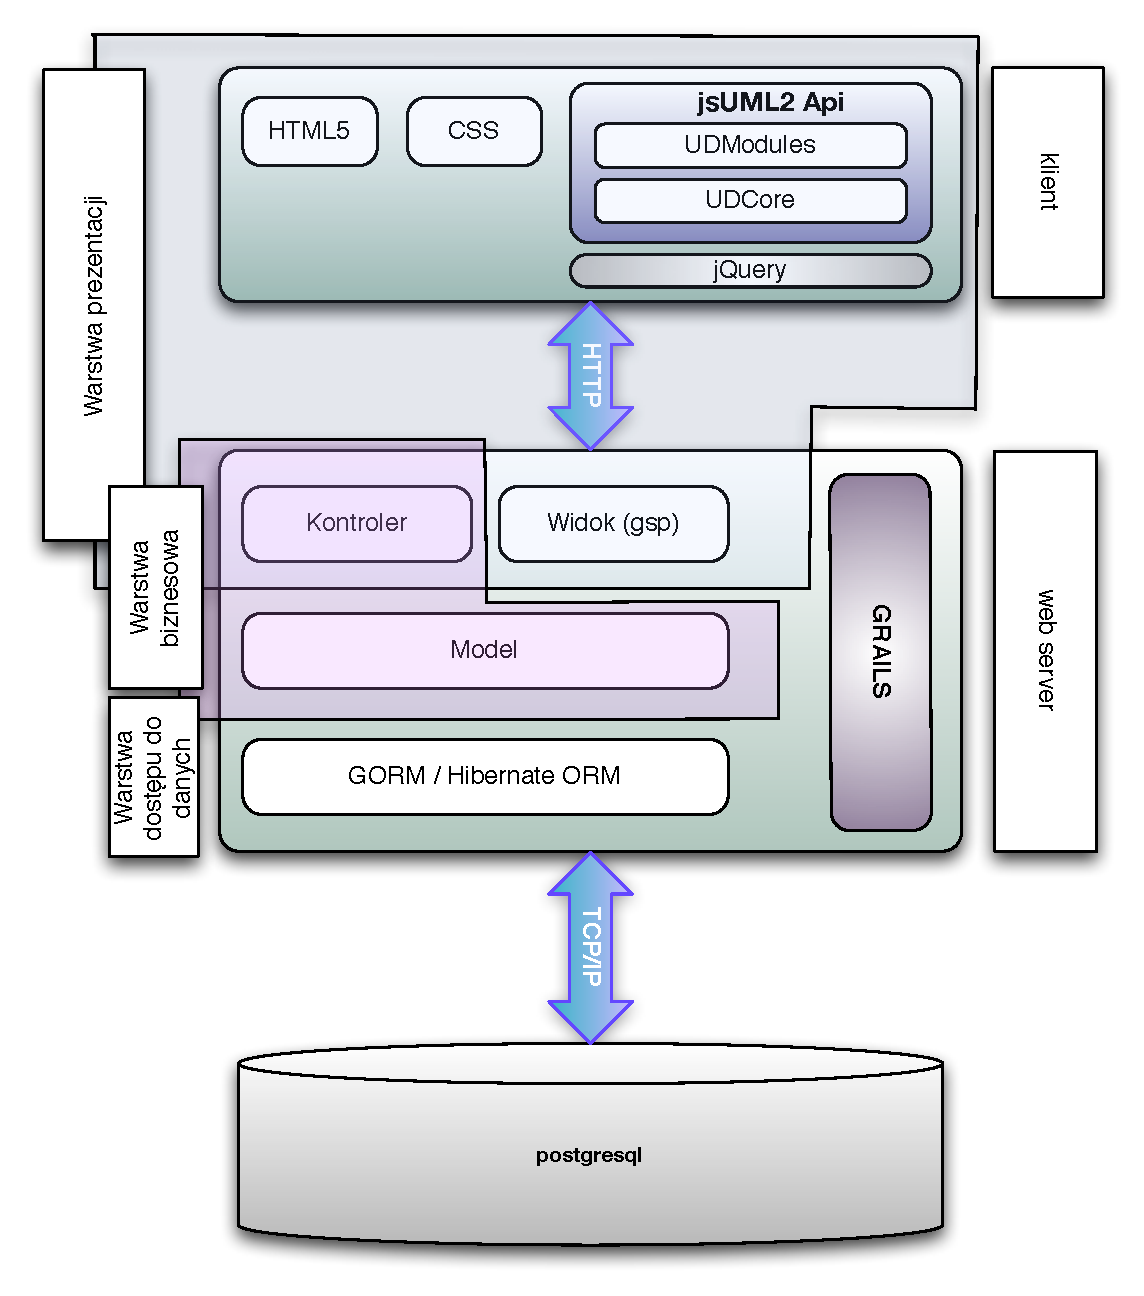
\includegraphics[width=1.0\textwidth]{img/reqmanager.pdf}
      \caption{Ogólna architektura systemu}
      \label{fig:reqarch}
    \end{figure*}

    \begin{verbatim}
    Diagram 
    Project
    Requirement
    UseCase
    \end{verbatim}

    Struktura bazy danych jest generowana automatycznie, na podstawie analizy klas modeli. Diagram utworzonej bazy, przedstawiono na rysunku \ref{fig:erd1}

    \begin{figure*}[p]
      \centering
      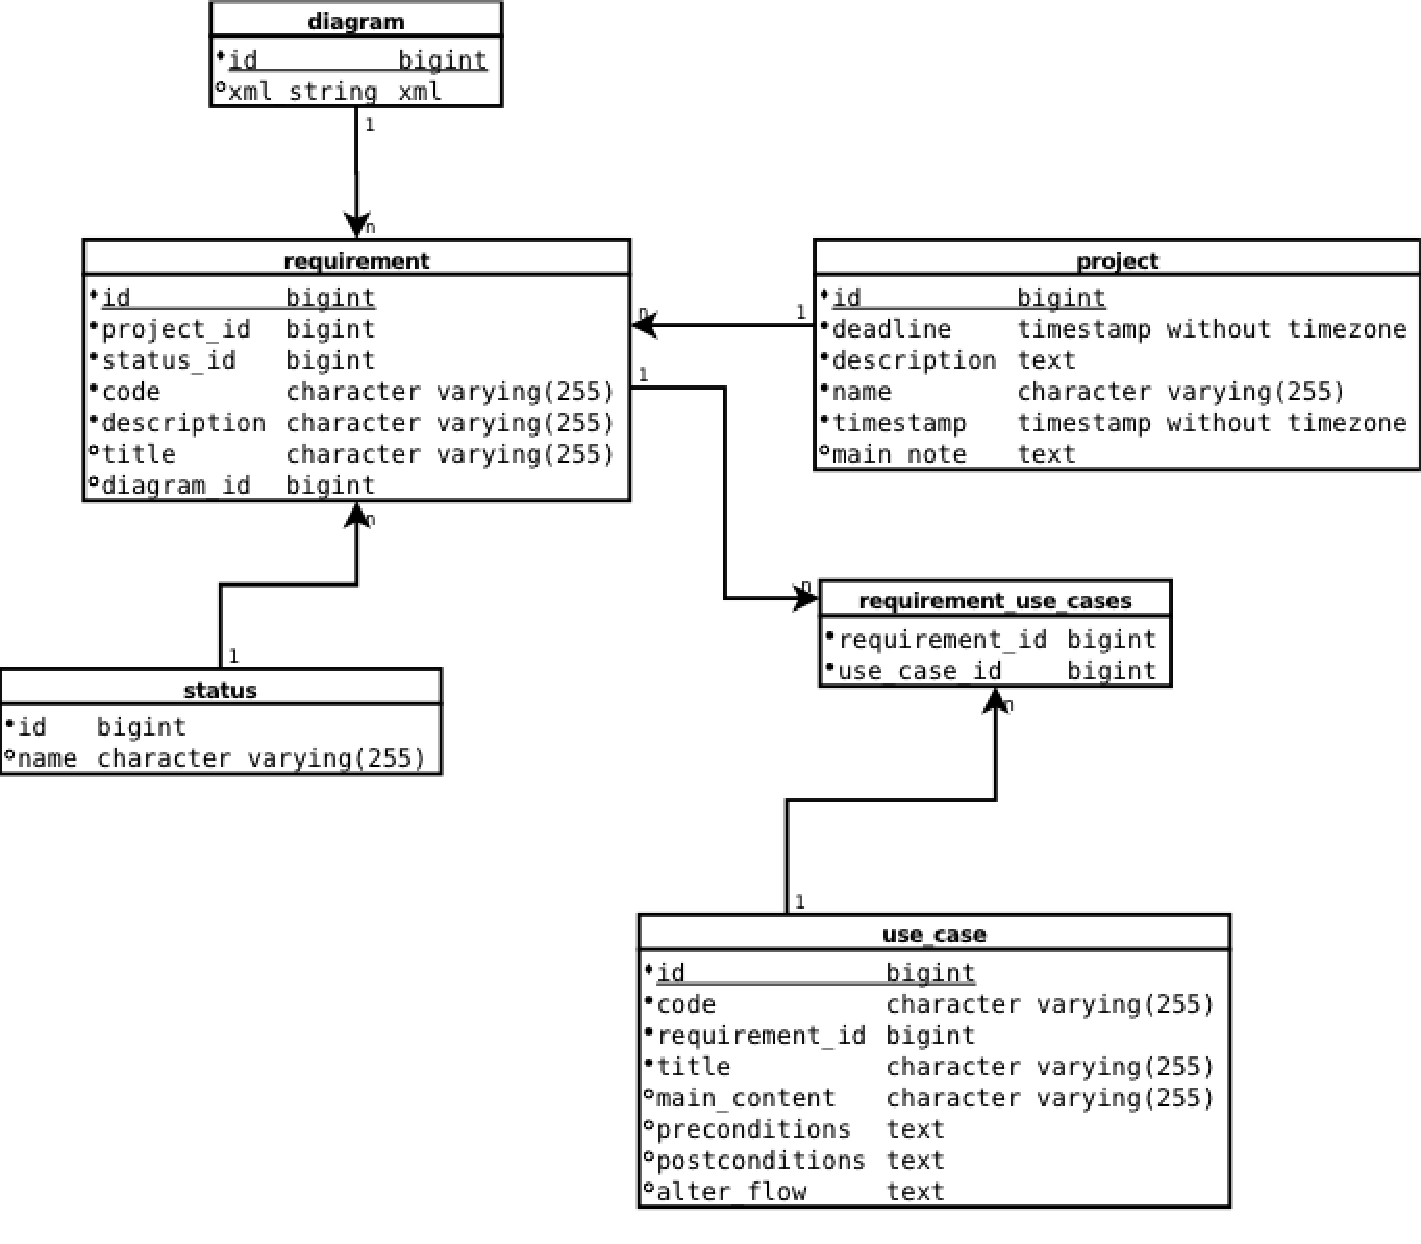
\includegraphics[width=1.0\textwidth]{img/erd2.pdf}
      \caption{Diagram struktury bazy danych systemu Reqmanager}
      \label{fig:erd1}
    \end{figure*}

  \section{Funkcjonalności systemu}

    Poniżej opisano poszczególne funkcjonalności proponowanego rozwiązania wraz z przykładami realizacji w kodzie.
  
    \subsection{Tworzenie diagramów}

      Diagramy przypadków użycia w systemie edytowane są po stronie klienta, dzięki wykorzystaniu elementu \emph{canvas} wprowadzonego niedawno do specyfikacji języka HTML5. Obsługa tej funkcjonalności po stronie przeglądarki, stanowi problem związany z zapisem stanu diagramu. W celu rozwiązania tego problemu, zaimplementowano mechanizm serializacji stanu elementów diagramu w formacie xml do bazy danych. Cel ten osiągnięto, wykorzystując metodę \emph{getXMLString()} udostępnioną przez wszystkie obiekty dziedziczące po klasie \emph{Diagram} w bibliotece jsUML2. Przykładową strukturę zserializowanego diagramu, umieszczono na Listingu \ref{lst:diagramXml}. 
      Dodanie nowego diagramu wiąże się zatem z inicjalizacją i wyświetleniem użytkownikowi obszaru roboczego diagramu bez komunikacji z serwerem. Diagram tworzony jest po załadowaniu widoku edycji wymagania, jak pokazano na Listingu \ref{lst:appUseCase}:

      \begin{lstlisting}[caption={Widok requriement/edit.gsp}, label={lst:appUseCase}]
      window.onload = function() {
        var app = new AppUseCase("ud_diagram_div");
      }

      \end{lstlisting}

      \newpage

      AppUseCase jest obiektem JavaScript typu singleton, którego skrócona implementacja została przedstawiona na Listingu \ref{lst:appUseCaseImpl}: 
    
      \begin{lstlisting}[caption={Implementacja obiektu JS AppUseCase}, label={lst:appUseCaseImpl}]
      var AppUseCase = function(elementId) { 
        var xmlstr = document.getElementById('diagramXml').value
        var ucDiag = new UMLUseCaseDiagram() 
        if(xmlstr) {
          ucDiag.setXMLString(xmlstr);
        }

        var c1 = document.getElementById('c1');
        var c = c1.getContext('2d');
        var c2 = document.getElementById('c2');
        c2.onmousedown = function() { return false; };
        var mc = c2.getContext('2d')}

        var div = document.getElementById('ud_diagram_div');

        ucDiag.initialize(11, div, c, mc, 600, 1000);
        ucDiag.draw();
      }
      \end{lstlisting}

      Powyższy kod JavaScript, pobiera wartość z elementu formularza i identyfikatorze ,,diagramXml'' oraz tworzy nowy obiekt UMLUseCaseDiagram, zdefiniowany w pakiecie \emph{modules} biblioteki jsUML2. Następnie weryfikuje czy pole \emph{diagramXml} jest niepuste. Jeśli warunek jest prawdziwy, wywołuje metodę \emph{setXMLString()} na obiekcie diagramu, dzięki czemu diagram inicjalizowany jest z wartościami wcześniej zserializowanymi do formatu xml i zapisanymi w bazie danych. Kolejne wiersze zajmują się utworzeniem kontekstów na bazie elementów \emph{canvas}, aby na końcu zainicjować i narysować odpowiedni diagram w oknie przeglądarki użytkownika. Należy jednocześnie zaznaczyć, iż w przypadku, gdy nie istnieje zserializowana wersja diagramu w bazie (pole \emph{diagramXml} jest puste), wówczas zostanie zainicjalizowany nowy, pusty diagram, nieposiadający żadnych elementów. 

      \subsubsection{Zapis danych xml}

      Dopiero gdy użytkownik wybierze opcję zapisu aktualnego wymagania, zserializowany stan diagramu w formacie xml, zostanie przesłany metodą POST do serwera. Następnie otrzymany po stronie serwera ciąg znaków xml zostanie przetworzony, utworzony zostanie obiekt klasy Diagram i na końcu nastąpi zapis obiektu do bazy danych. Za ten proces odpowiedzialna jest akcja \emph{save} kontrolera \emph{Requirement}. Jest to dość ograniczone rozwiązanie, które można byłoby usprawnić wprowadzając asynchroniczny, automatyczny zapis stanu diagramu co kilka sekund lub po każdej aktualizacji po stronie klienta.

      \begin{lstlisting}[caption={Struktura xml diagramu}, label={lst:diagramXml}]

      <UMLUseCaseDiagram name="Use case diagram">
        <UMLSystem id="UMLSystem_4" x="165" y="97" ... >
          <superitem id="stereotypes" visibleSubComponents="true"/>
          <item id="name" value="System name"/>
          <UMLUseCase id="UMLUseCase_1" x="232" y="142" ... >
            <superitem id="stereotypes" visibleSubComponents="true"/>
            <item id="name" value="test test"/>
          </UMLUseCase>
          <UMLUseCase id="UMLUseCase_3" x="222" y="209" ... >
            <superitem id="stereotypes" visibleSubComponents="true"/>
            <item id="name" value="for req 74"/>
          </UMLUseCase>
        </UMLSystem>
      </UMLUseCaseDiagram>

      \end{lstlisting}

      Baza danych PostgreSQL obsługuje specjalny typ danych ,,xml''. Dzięki temu, po stronie bazy dokonywana jest weryfikacja poprawności dokumentu jaki programista ma zamiar zapisać. Niestety Framework Grails nie współpracuje dobrze z taką konstrukcją, dlatego niezbędna była implementacja rozwiązania rzutującego typ \emph{String} na typ \emph{SQLXMLType}. W tym celu została stworzona specjalna klasa w Javie, implementująca interfejs \emph{org.hibernate.usertype.UserType} (patrz Listing \ref{lst:xmlType}). Hibernate udostępnia ten interfejs umożliwiając programistom tworzenie własnych typów danych i zdefiniowanie ich zachowania w stosunku do bazy. Dodatkowo, niezbędne było odpowiednie przygotowanie modelu, podając typ pola przechowującego xml jako String, a następnie stworzyć odpowiedni blok ,,mapping'' w modelu. Na Listingu \ref{lst:xml}, dla przykładu zaprezentowano implementację klasy Diagram z systemu Reqmanager:
 
      \begin{lstlisting}[caption={Implementacja niestandardowego typu SQLXMLType}, label={lst:xmlType}]
      package pl.edu.pjwstk.reqmanager
       
      import java.io.Serializable;
      import java.sql.PreparedStatement;
      import java.sql.ResultSet;
      import java.sql.SQLException;
      import java.sql.Types;
      import org.hibernate.HibernateException;
       
      /**
       * Store and retrieve a PostgreSQL "xml" column as a Java string.
       */
      public class SQLXMLType implements org.hibernate.usertype.UserType {
       
          private final int[] sqlTypesSupported = new int[] { Types.VARCHAR };
       
          @Override
          public int[] sqlTypes() {
              return sqlTypesSupported;
          }
       
          @Override
          public Class returnedClass() {
              return String.class;
          }
       
          @Override
          public boolean equals(Object x, Object y) throws HibernateException {
              if (x == null) {
                  return y == null;
              } else {
                  return x.equals(y);
              }
          }
       
          @Override
          public int hashCode(Object x) throws HibernateException {
              return x == null ? null : x.hashCode();
          }
       
          @Override
          public Object nullSafeGet(ResultSet rs, String[] names, Object owner) throws HibernateException, SQLException {
              assert(names.length == 1);
              String xmldoc = rs.getString( names[0] );
              return rs.wasNull() ? null : xmldoc;
          }
       
          @Override
          public void nullSafeSet(PreparedStatement st, Object value, int index) throws HibernateException, SQLException {
              if (value == null) {
                  st.setNull(index, Types.OTHER);
              } else {
                  st.setObject(index, value, Types.OTHER);
              }
          }
       
          @Override
          public Object deepCopy(Object value) throws HibernateException {
              if (value == null)
                  return null;
              return new String( (String)value );
          }
       
          @Override
          public boolean isMutable() {
              return false;
          }
       
          @Override
          public Serializable disassemble(Object value) throws HibernateException {
              return (String) value;
          }
       
          @Override
          public Object assemble(Serializable cached, Object owner) throws HibernateException {
              return (String) cached;
          }
       
          @Override
          public Object replace(Object original, Object target, Object owner) throws HibernateException {
              return original;
          }
      }
      \end{lstlisting}

      \newpage

      \begin{lstlisting}[caption={Implementacja modelu Diagram}, label={lst:xml}]
      package pl.edu.pjwstk.reqmanager
      public class Diagram {
        String name
        String xmlString

        static belongsTo = Requirement
        static mapping = {
          xmlString type: SQLXMLType
        }
        static constraints = {
          name(nullable:true)
        }
      }
      \end{lstlisting}

    \subsection{Współdzielenie diagramów}

    Istotnym elementem systemu jest współdzielenie diagramów między wieloma wymaganiami. Każdy diagram może zostać przypisany do kilku wymagań. Wówczas modyfikacja przypadków użycia w trakcie edycji konkretnego wymagania, wiąże się z aktualizacją stanu diagramu we wszystkich korzystających z niego miejscach w systemie.
    
    \subsection{Mapowanie przypadków użycia}
      W związku z możliwością współdzielenia diagramów pomiędzy wieloma wymaganiami, w aktualnej wersji prototypu, przypadki użycia są łączone z wymaganiem, tylko po wykonaniu przez użytkownika akcji wskazania przypadku użycia jako realizującego aktualnie modyfikowane wymaganie.

      Na etapie edycji diagramu, użytkownik ma możliwość wskazania konkretnych use case'ów znajdujących się na diagramie, jako odpowiedzialnych za realizację wybranego wymagania. Powiązanie przypadku użycia z wymaganiem polega na wyborze opcji \emph{mark for requirement} z paska narzędzi diagramu, a następnie kliknięciu w dany przypadek użycia na diagramie. Po zatwierdzeniu operacji, zostaje wysłane asynchroniczne żądanie do serwera, pod adres http://reqmanager.herokuapp.com/requirement/\\addUseCase/id\_wymagania. W żądaniu przekazywane są do serwera parametry niezbędne dla zestawienia przypadku użycia z wymaganiem. Poniżej zamieszczono listę tych parametrów:

    \begin{itemize}
      \item \emph{id} - identyfikator wymagania do którego dodawany jest przypadek użycia
      \item \emph{clickedUCName} - nazwa przypadku użycia wprowadzona przez użytkownika
      \item \emph{clickedUCId} - identyfikator przypadku użycia wygenerowany automatycznie przez bibliotekę jsUML2
    \end{itemize}

    Asynchronicznie wysłane do serwera żądanie zostaje przekazane wraz z paramterami do akcji \emph{addUseCase} kontrolera \emph{Requirement}. Kod odpowiedzialny za połączenie przypadku użycia z wymaganiem, został załączony na Listingu \ref{lst:addUseCase}.

    \begin{lstlisting}[caption={Kod łączący przypadek użycia z wymaganiem}, label={lst:addUseCase}]
    def addUseCase = {
      def requirement = Requirement.get(params.id)
      def useCase = UseCase.findByTitle(params.clickedUCName)
      if(useCase == null) {
        useCase = new UseCase(title: params.clickedUCName, code: params.clickedUCId)
          requirement.addToUseCases(useCase)
          render(text: "ok")
      } else {
        if(!requirement.useCases.contains(useCase)) {
          requirement.addToUseCases(useCase)
          render(text: "ok")
        } 
      }
    }
    \end{lstlisting}

    Jak można odczytać z powyższego kodu źródłowego, akcja ta, pobiera odpowiednie wymaganie oraz podejmuje próbę znalezienia przypadku użycia po nazwie. Jeśli dany przypadek użycia nie istnieje jeszcze w bazie danych (nowo utworzony przypadek użycia), zostaje swtorzony nowy obiekt klasy UseCase z odpowiednimi parametrami (nazwa nadana przez użytkownika oraz identyfikator wygenerowany po stronie klienta). W przeciwnym razie, zostaje on dodany do listy przypadków użycia połączonych asocjacją z danym wymaganiem, o ile nie istnieje już na tej liście. 

    \subsection{Przypadki użycia a wymagania}
    
      W celu odpowiedniego oznaczenia przypadków użycia przypisanych do wybranego wymagania, zaimplementowano algorytm dwustopniowej inicjalizacji diagramu. Pierwszym krokiem jest ekstrakcja z bazy danych odpowiedniego wymagania, weryfikacja czy jest do niego przypisany diagram oraz czy istnieją dla niego jakieś przypadki użycia. Na podstawie tych informacji, ładowany jest widok \emph{requirement/show.gsp}. Następnie, po załadowaniu strony uruchamiany jest skrypt po stronie klienta, odwołujący się asynchronicznie z powrotem do serwera z ,,pytaniem'' o nazwy przypadków użycia przypisanych do danego wymagania. Następnie, do pamięci ładowana jest struktura xml diagramu. Program iteruje po wszyskich węzłach w poszukiwaniu pokrywających się przypadków użycia. Jeśli znajdzie choć jeden, zmienia kolor jego tła na żółty. Listing \ref{lst:colorUC} przedstawia implementację tego algorytmu.
      
    
    \begin{lstlisting}[caption={Mechanizm oznaczania przypadku użycia przypisanego do aktualnie otwartego wymagania}, label={lst:colorUC}]
    var reqUseCases = $.ajax({
      type: "GET",
      url: "http://reqmanager.herokuapp.com/requirement/getUseCases/" + reqId,
      cache: false
    }).done(function(xht){ 
      var dom = (new DOMParser()).parseFromString(diag.diagram.getXMLString(), "text/xml");
      var documentEle = dom.documentElement;
      var usecaseArray = documentEle.getElementsByTagName('UMLUseCase');

      for(var i = 0; i < usecaseArray.length; i++) {
        for(var j = 0; j < usecaseArray[i].childNodes.length; j++) {
          var itemValue = usecaseArray[i].childNodes[j].attributes.value;
          if(itemValue != undefined) {
            if(xht.indexOf(itemValue.value.toString()) != -1) {
              var divv = document.getElementById("ud_diagram_div");
              var foundUseCase = null;

              for(var k = 0; k < diag.diagram._nodes.length; k++) {
                if(diag.diagram._nodes[k].getName().toString() 
                  === xht[xht.indexOf(itemValue.value.toString())]) {
                  foundUseCase = diag.diagram._nodes[k]; 
                }
              };
              if(foundUseCase) foundUseCase.setBackgroundColor("#F3F5BC");
              diag.diagram.draw();
            }
          }
        }
      }
    });
    \end{lstlisting}

    \newpage

    \subsection{Edytor tekstu}
      W celu ułatwienia użytkownikowi pracy z tekstem, zaimplementowano edytor, oparty na bibliotece Ace Editor. 
      Kod inicjujący edytor tekstu, znajduje się na Listingu \ref{lst:editorInit}.

    \begin{lstlisting}[caption={Inicjalizacja edytora tekstu}, label={lst:editorInit}]
    var editor = ace.edit("description");
    var MarkdownMode = require("ace/mode/markdown").Mode;
    editor.setTheme("ace/theme/clouds_midnight");
    editor.getSession().setMode(new MarkdownMode());
    editor.getSession().setUseWrapMode(true);
    \end{lstlisting}

    Kod z Listingu \ref{lst:editorInit} inicjuje edytor, załączając go do wskazanego węzła w dokumencie html (w tym przypadku jest to warstwa ,,description''). Następnie ustawia wygląd graficzny edytora oraz przestawia go w tryb pracy z formatem Markdown.
    Zawartość edytora tekstu, przekazywana jest do serwera po wysłaniu formularza przez użytkownika. Ponieważ zawartość formularza znajduje się w elemencie \emph{div} w strukturze DOM strony, w celu przekazania jego wartości, jest ona kopiowana do specjalnego pola typu textarea. Proces ten zaprezentowano na Listingu \ref{lst:txtCopy}.

    \begin{lstlisting}[caption={Kopiowanie zawartości edytora tekstu do pola textarea}, label={lst:txtCopy}]
    $("#submitbtn").click(function() {
      textarea.val(editor.getSession().getValue()); 
      $("#diagramXml").val(app.diagram.getXMLString());
    });
    \end{lstlisting} 

    \subsection{Generowanie dokumentacji}
      
      W prototypie zaimplementowano mechanizm generowania specyfikacji wymagań przy użyciu bibliotek MarkdownJ oraz iText.

      MarkdownJ jest napisaną w Javie implementacją konwertera tekstu do formatu HTML. Jest to bardzo prosta biblioteka, w której główną klasą jest \emph{MarkdownProcessor}. Metoda \emph{markdown()} przymuje jako parametr ciąg znaków (sformatowany znacznikami Markdown). W odpowiedzi zwracana jest ta sama treść, osadzona w odpowiedniej strukturze HTML. Przykładowy kod konwertujący przedstawiono na Listingu \ref{lst:markdownProc}.

      \begin{lstlisting}[caption={Wykorzystanie klasy MarkdownProcessor}, label={lst:markdownProc}]
      def m = new MarkdownProcessor(); 
      StringBuffer sb = new StringBuffer()
      sb.append("# Example header in Markdown")
      sb.append("\n")
      sb.append("This will render as a regular '<p>' paragraph")
      String html = m.markdown(sb.toString()); 
      \end{lstlisting}

      iText z kolei, jest zaawansowaną biblioteką wykorzystywaną do generowania wszelkiego rodzaju dokumentów PDF bezpośrednio z kodu Javy. W pracy wykorzystano klasę \emph{ITextRenderer} dostępną w pakiecie org.xhtmlrenderer.pdf. Pozwala ona na generowanie dokumentów PDF w oparciu o strukturę XHTML. Połączenie MarkdownJ z biblioteką iText idealnie spełnia wymagania systemu w zakresie automatycznego tworzenia specyfikacji.

      Generowanie specyfikacji w systemie przebiega w dwóch krokach. W pierwszej kolejności zostają pobranie niezbędne informacje z bazy danych dotyczące wybranego projektu, a zawartość poszczególnych pól, zostaje przekazana do klasy MarkdownToHTML konwertującej tekst do HTML. Następnie, zwrócona struktura jest przekazywana klasie ITextRenderer w celu wygenerowania dokumentu PDF. Zwrócony strumień danych zostaje wysłany do klienta jako odpowiedź serwera, co skutkuje możliwością zapisu pliku PDF na komputerze klienckim. Proces ten zobrazowany został na diagramie sekwencji, załączonym na Rysunku \ref{fig:seq}.

      \begin{figure*}[t]
        \centering
        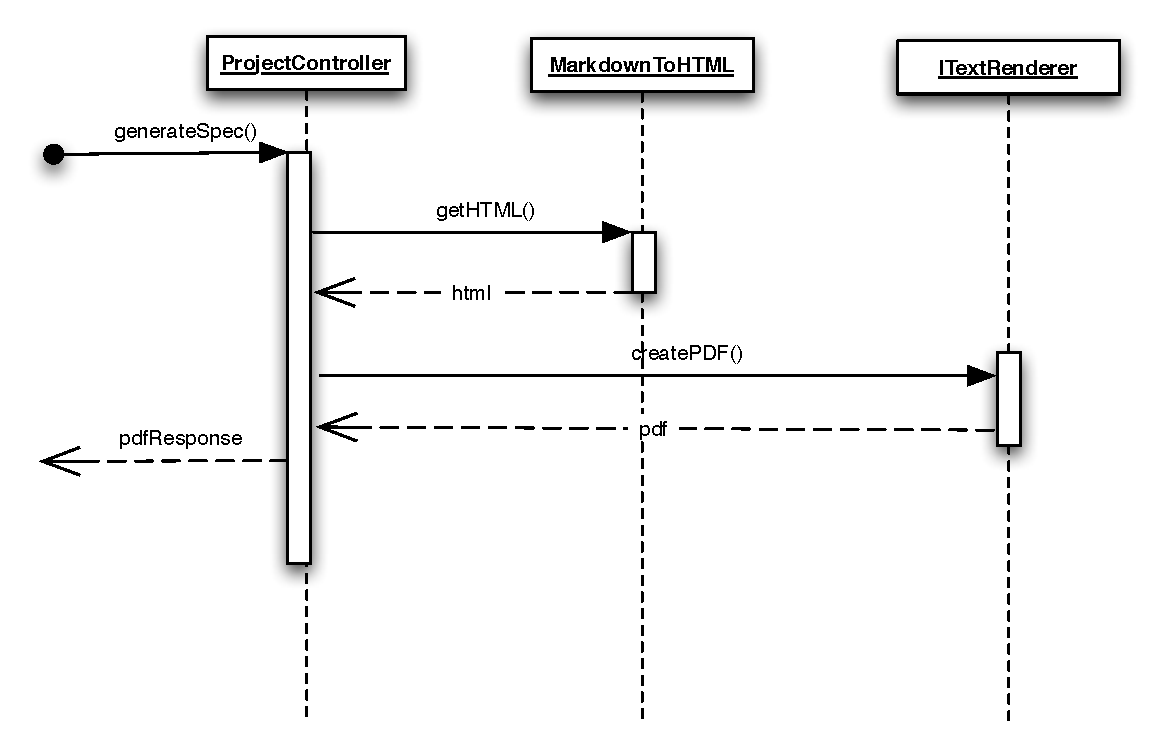
\includegraphics[width=1.0\textwidth]{img/seq.pdf}
        \caption{Generowanie dokumentu pdf specyfikacji}
        \label{fig:seq}
      \end{figure*}

      \newpage

  \section{Przykład zastosowania}
    
    W tej sekcji opisano przykład zastosowania proponowanego narzędzia.

    \subsection{Ekran główny}
      
      Ekranem głównym systemu jest przegląd wszystkich projektów, przedstawiony na Rysunku \ref{fig:mainView}. Przy każdym projekcie zawarte są podstawowe informacje na jego temat, takie jak nazwa, data zakończenia, krótki opis, ilość wymagań oraz przypadków użycia. Ponadto dostępne są trzy przyciski: (1) odnośnik do szczegółów projektu, (2) odnośnik do edycji projektu, (3) przycisk generujący aktualną wersję specyfikacji wymagań. 

      \begin{figure*}[t]
        \centering
        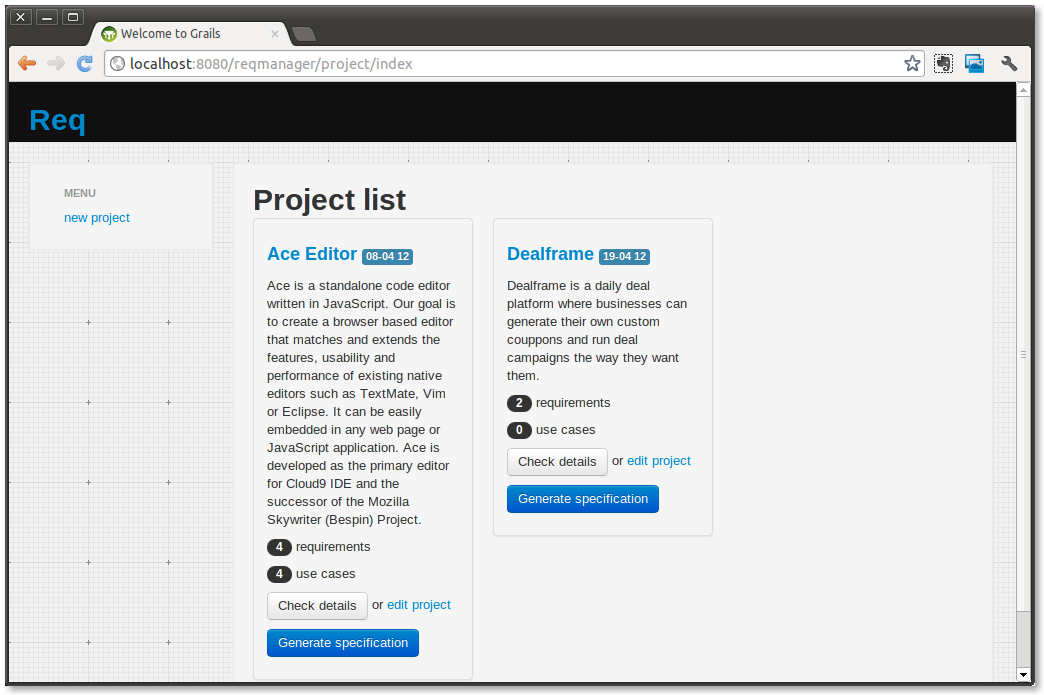
\includegraphics[width=1.0\textwidth]{img/tut_screen_1.png}
        \caption{Ekran główny projektu}
        \label{fig:mainView}
      \end{figure*}

    \subsection{Nowy projekt}
    
      Dodanie nowego projektu polega na wypełnieniu prostego formularza zawierającego informacje o nazwie, dacie zakończenia prac, krótkim opisie oraz głównej notatce. Rysunek \ref{fig:addProj} przedstawia ekran zakładania projektu.

      \begin{figure*}[t]
        \centering
        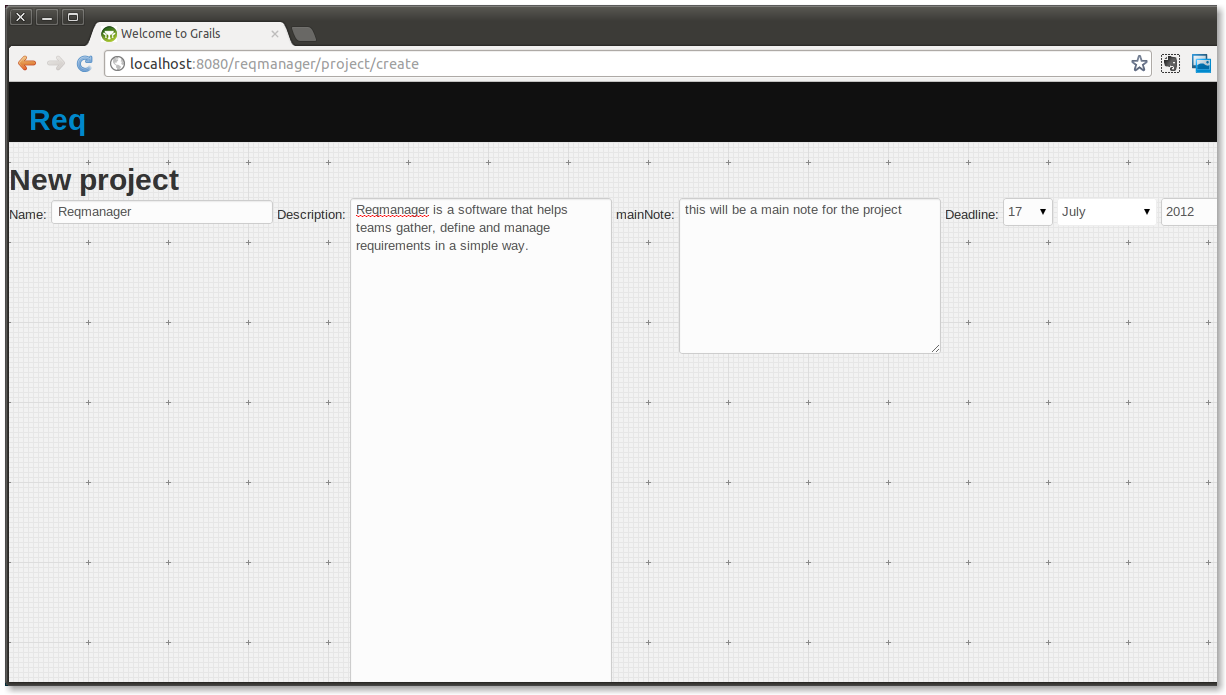
\includegraphics[width=1.0\textwidth]{img/tut_2.png}
        \caption{Dodawanie nowego projektu}
        \label{fig:addProj}
      \end{figure*}

    \subsection{Pierwsze wymaganie}

      Do nowo utworzonego projektu, można natychmiast rozpocząć dodawanie wymagań. Widok dodawania pierwszego wymagania załączono na Rysunku \ref{fig:addReq}. W tym miejscu, użytkownik ma możliwość podjęcia decyzji dotyczącej ponownego wykorzystania już istniejącego diagramu lub stworzenia nowego. Rysunek \ref{fig:addReq} przedstawia stan aplikacji po stworzeniu nowego diagramu, dodaniu pierwszego aktora, elementu granicy systemu i jednego przypadku użycia. W kolejnych widokach zaprezentowano współdzielenie diagramów.

      \begin{figure*}[t]
        \centering
        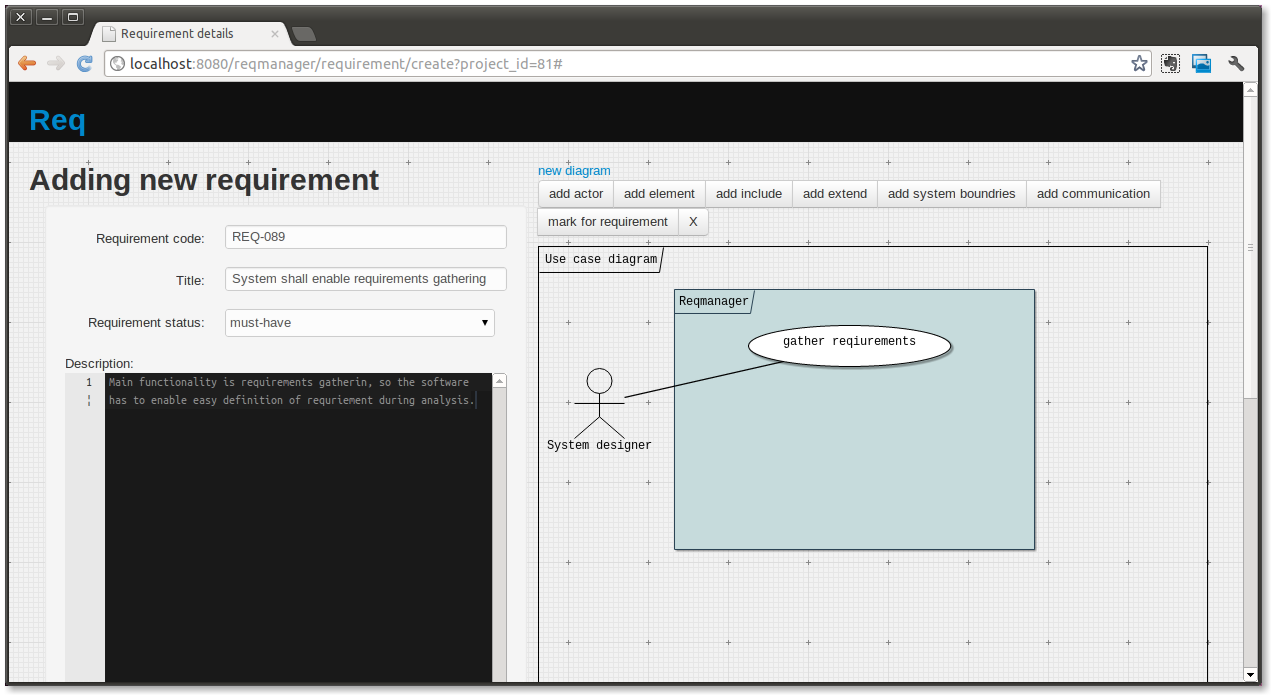
\includegraphics[width=1.0\textwidth]{img/tut_3.png}
        \caption{Definicja wymagania}
        \label{fig:addReq}
      \end{figure*}

    \subsection{Przegląd projektu}

      Rysunek \ref{fig:afterAddReq} przedstawia stan systemu po dodaniu jednego wymagania. Za pośrednictwem tego ekranu, użytkownik ma możliwość kontynuacji pracy nad główną notką projektową (i łatwy zapis tego pola za pomocą przycisku ,,Update'' umieszczonego w widocznym, dostępnym miejscu) lub dodania kolejnego wymagania.

      \begin{figure*}[t]
        \centering
        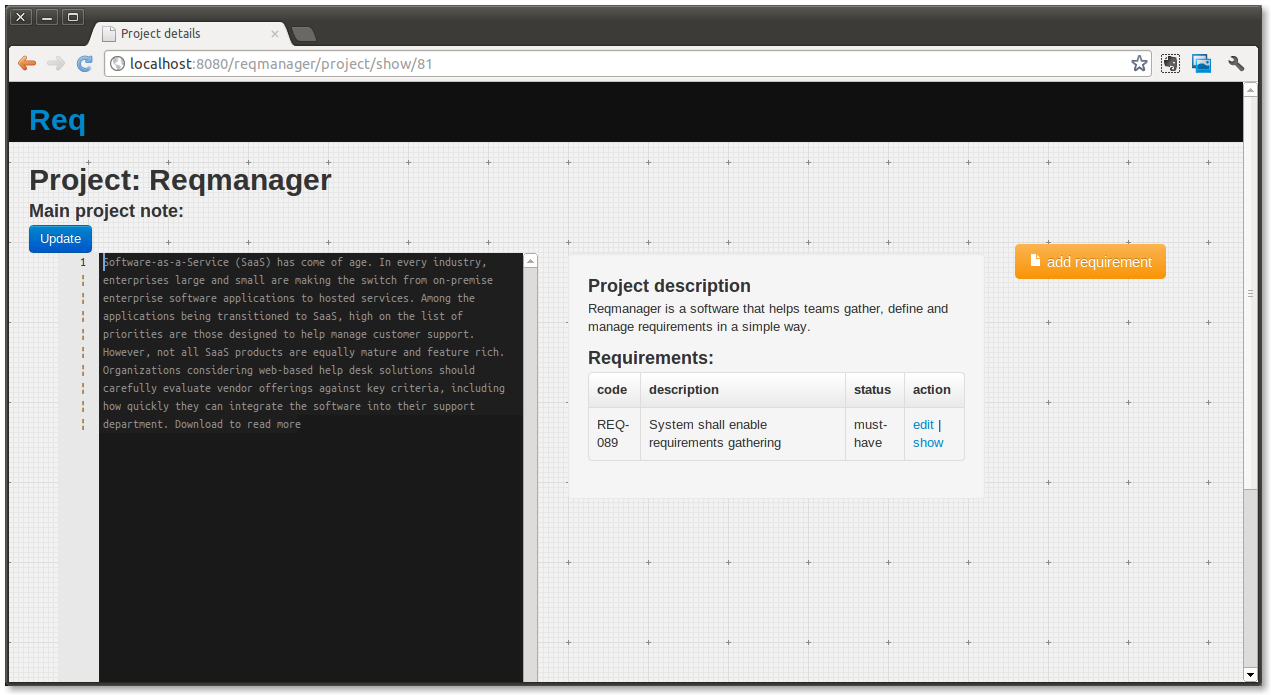
\includegraphics[width=1.0\textwidth]{img/tut_4.png}
        \caption{Stan systemu po dodaniu pierwszego wymagania}
        \label{fig:afterAddReq}
      \end{figure*}
      
    \subsection{Współdzielenie wymagań}

      Podczas dodawania kolejnych wymagań, użytkownik ma możliwość skorzystania z już istniejącego diagramu, co zaprezentowano na Rysunku \ref{fig:diagReuse}. Zamiast tworzenia nowej instancji diagramu, użytkownik ma możliwość wskazania istniejącego obiektu, który zostanie przypisany do aktualnie definiowanego elementu. Rysunek \ref{fig:diagReuse} zawiera również przykład zastosowania podstawowej składni Markdown w opisie wymagania.

      \begin{figure*}[t]
        \centering
        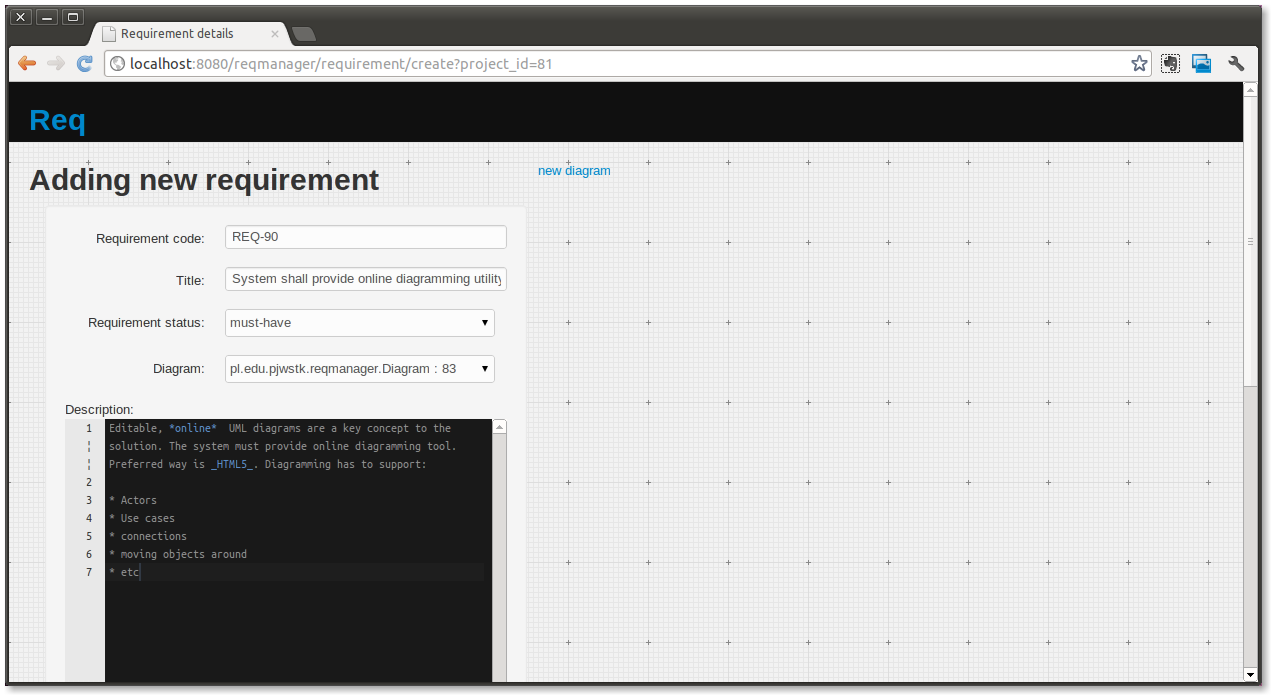
\includegraphics[width=1.0\textwidth]{img/tut_8.png}
        \caption{Współdzielenie diagramu}
        \label{fig:diagReuse}
      \end{figure*}

    \subsection{Łączenie przypadków użycia z wymaganiem}

      Wracając do widoku przedstawionego na Rysunku \ref{fig:addReq}, należy zwrócić uwagę na przycisk ,,mark for requirement'' w pasku narzędzi edytora UML. Wybierając tę opcję, a następnie wskazując wybrany przypadek użycia na diagramie, zostaje wykonana asynchronicznie operacja połączenia use case'u z wymaganiem. Po przejściu do podglądu wymagania, przypisane do niego przypadki użycia są zaznaczane kolorem żółtym. Właściwość ta, została zaprezentowana odpowiednio na Rysunkach \ref{fig:reqShow1} oraz \ref{fig:reqShow2}.

      \begin{figure*}[t]
        \centering
        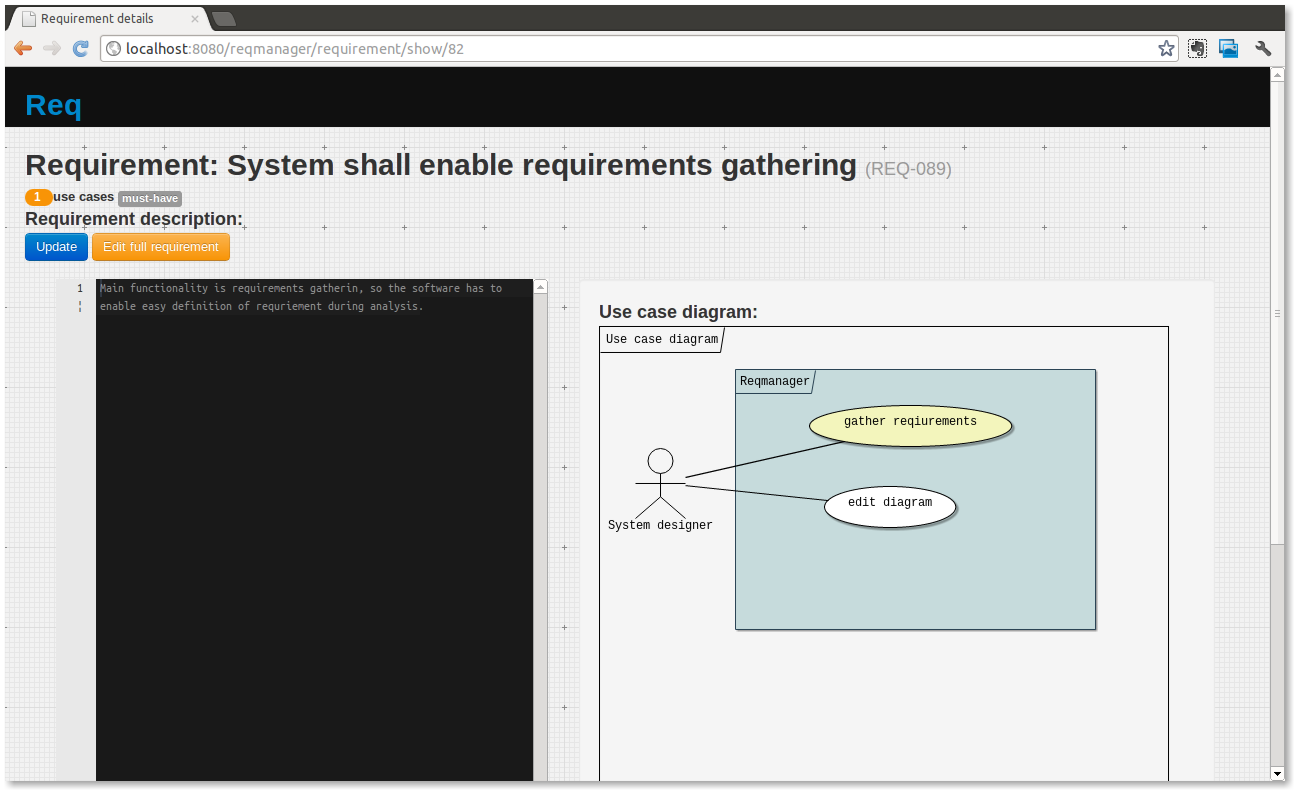
\includegraphics[width=1.0\textwidth]{img/tut_11.png}
        \caption{Jeden przypadek połączony z wymaganiem}
        \label{fig:reqShow1}
      \end{figure*}
      \begin{figure*}[t]
        \centering
        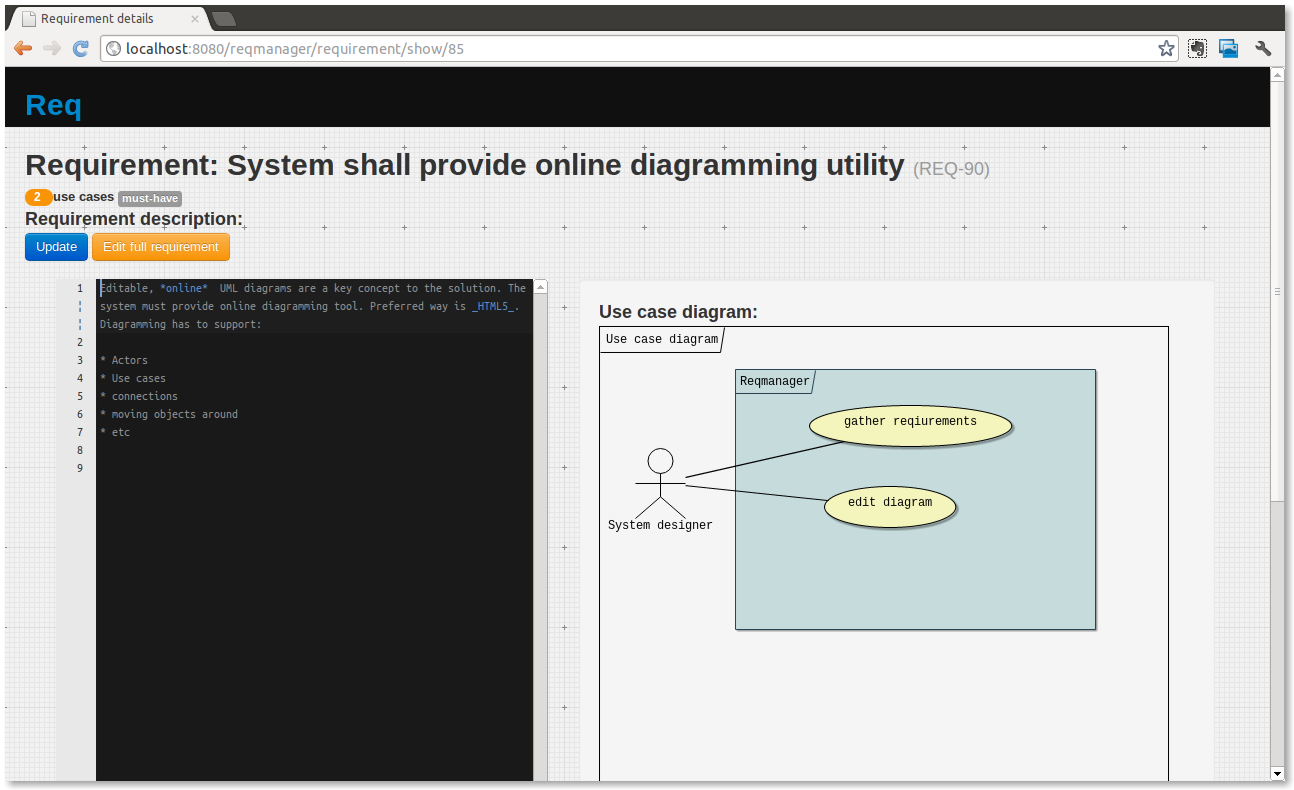
\includegraphics[width=1.0\textwidth]{img/tut_10.png}
        \caption{Dwa przypadki użycia połączone z wymaganiem}
        \label{fig:reqShow2}
      \end{figure*}

    \subsection{Generowanie specyfikacji}

      W każdym momencie prac nad analizą, użytkownicy mają możliwość wygenerowania aktualnej specyfikacji wymagań z ekranu głównego aplikacji. Proces polega wyłącznie na wybraniu opcji ,,Generate specification''. System analizuje dane wprowadzone do bazy i na ich podstawie generuje dokument PDF, który jest przekazywany do przeglądarki klienckiej. Wynik wygenerowania specyfikacji dla projektu powstałego na potrzeby powyższych przykładów pokazano na Rysunku \ref{fig:spec}.

      \begin{figure*}[t]
        \centering
        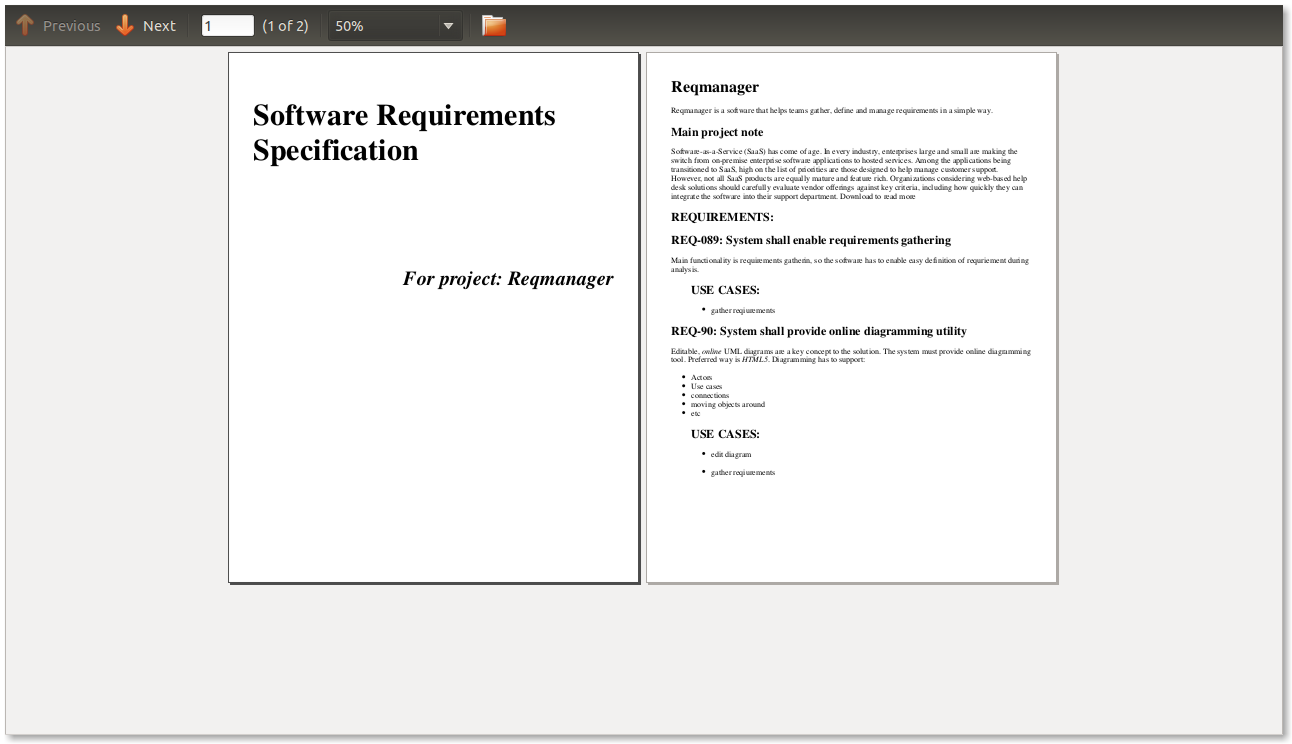
\includegraphics[width=1.0\textwidth]{img/tut_9.png}
        \caption{Wygenerowana specyfikacja wymagań w PDF}
        \label{fig:spec}
      \end{figure*}

  \newpage

  \section{Zalety i wady proponowanego rozwiązania}
    Proponowane rozwiązanie jest podjęciem próby uproszczenia procesów inżynierii wymagań. Głównym celem stworzenia prototypu było dostarczenie narzędzia umożliwiającego efektywne zbieranie i przetwarzanie wymagań przy jednoczesnym uproszczeniu poziomu jego skomplikowania. Powstał prototyp realizujący te cele, jednak siłą rzeczy, jest to narzędzie przystosowane jedynie do małych projektów. W przeciwieństwie do istniejących rozwiązań, filozofia proponowanego systemu inspirowana była filozofią systemów Unix - programy i aplikacje powinny wykonywać jedną czynność i powinny ją wykonywać możliwie najlepiej. Jednocześnie należy tworzyć aplikacje tak, aby mogły w łatwy sposób współpracować z innymi systemami. Dlatego proponowane rozwiązanie, aby rozwiązywało skutecznie problemy ogólnie pojętej inżynierii oprogramowania, powinno być stosowane komplementarnie z innymi narzędziami, w szczególności systemem zarządzania projektami i zespołem. Od świadomości i dojrzałości organizacji zależy, jak taka infrastruktura zostanie zbudowana oraz jak wybrane narzędzia będą funkcjonowały w organizacji.

    Dużą zaletą systemu jest dostępność przez przeglądarkę internetową przy jednoczesnej realizacji funkcjonalności manipulacji obiektami graficznymi. W szczególności zastosowanie technologii HTML5 daje przewagę w dostępności nad istniejącymi rozwiązaniami, najczęściej implementowanymi w technologii Flash. Rzadko też można spotkać podobny poziom elastyczności aplikacji do zarządzania wymaganiami. Koncepcja systemu celowo nie narzuca wielu ograniczeń związanych ze strukturą wymagań w wierze, że brak restrykcji projektanta wpłynie pozytywnie na proces definiowania i formułowania wymagań. 

    Sam wybór technologii jaką jest Grails, jest zaletą stworzonego prototypu. Zastosowanie tej technologii umożliwia łatwą rozbudowę i skalowanie systemu. System wtyczek platformy Grails sprzyja modułowej naturze aplikacji stworzonych w tej technologii. Z kolei zarządzający całą aplikacją ,,silnik'' oparty na String Framework, Hibernate ORM oraz filozofii ,,convention over configuration'' sprzyjają stosowaniu najlepszych praktyk programistycznych i ponowne wykorzystanie kodu.

    Z pewnością istotną wadą jest brak obsługi ,,śledzenia'' wymagań (traceability). Jednak w istniejących rozwiązaniach śledzenie wymagań nie rozwiązuje w pełni problemu. Nadal należy dbać o zgodność kodów i identyfikatorów wymagań w komunikacji z wieloma systemami. W dobrze zorganizowanej firmie, te problemy można wyeliminować przez narzucenie odpowiedniej kultury pracy, dbałość o szczegóły i skrupulatność w raportowaniu implementowanych rozwiązań do różnych systemów, jednak dopóki istnieje wiele narzędzi wspomagających różne etapy w procesie wytwórczym, odpowiednia komunikacja i wymiana danych jest jedyną metodą umożliwiającą skuteczne śledzenie wymagań.
